\section{Initial Gene Finding Results}\label{section:gene-finding}

Prior to discussing gene finding results, we will first define the
terms gene and coding sequence in the context of this work. We refer
to a gene as a set of start and stop coordinates in a genomic
sequence. This definition of a gene simplifies processing, although
the definition could be expanded in the future to include introns,
exons and potential up and downstream sequences as well. Gene finders
may also predict isoforms, or alternative splice variants of a gene
based on evidence provided in training, resulting in multiple
potential coding sequences for a gene. In this work, we refer to
coding sequences as the set of all coding sequences predicted by a
gene finder.

Counts of genes and coding sequences predicted by Braker2, GeneMark
and RefSeq are shown in Figure~\ref{fig:gene-counts},
Figure~\ref{fig:cds-counts} and
Table~\ref{table:gene-counts}. Immediately we see that Braker2
predicts far fewer genes in all assemblies, except in the case of
\textit{Trichoderma reesei.} This is possibly due to the effects of
training the Braker2 gene model using data from \textit{Trichoderma
  reesei}, which has a significantly smaller genome in comparison to
other \textit{Trichoderma} assemblies, although genome size is not
always indicative of gene content. Regardless, we observe a difference
in the number of genes predicted by Braker2 in comparison to GeneMark
and RefSeq. The number of genes predicted by GeneMark and RefSeq are
similar, except in the case of \textit{T. harzianum}, in which RefSeq
predicts roughly 17\% more genes than GeneMark. Braker2 consistently
predicts more coding sequences than GeneMark and RefSeq. RefSeq also
appears to predict multiple coding sequences for each gene but in
fewer numbers than Braker2. Coding sequence prediction counts in
\textit{T. harzianum} from RefSeq are also interesting, with RefSeq
predicting fewer coding sequences than genes. Why this occurs is
unknown but may warrant further investigation.

\begin{figure}
  \centering
  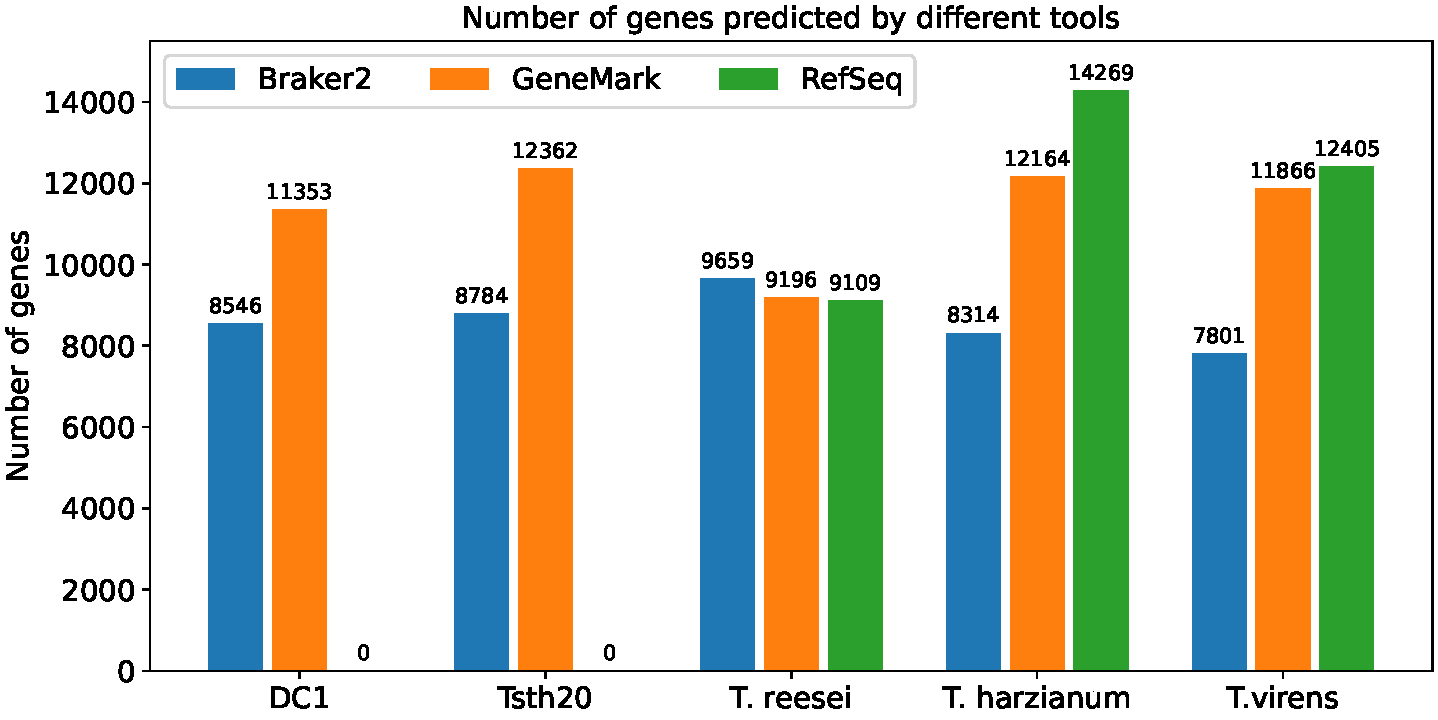
\includegraphics[width=0.9\textwidth]{figures/gene-counts-barplot.pdf}
  \caption[Number of genes predicted]{Number of genes predicted by each gene finder for each \textit{Trichoderma} genome assembly.}\label{fig:gene-counts}
\end{figure}

\begin{figure}
  \centering
  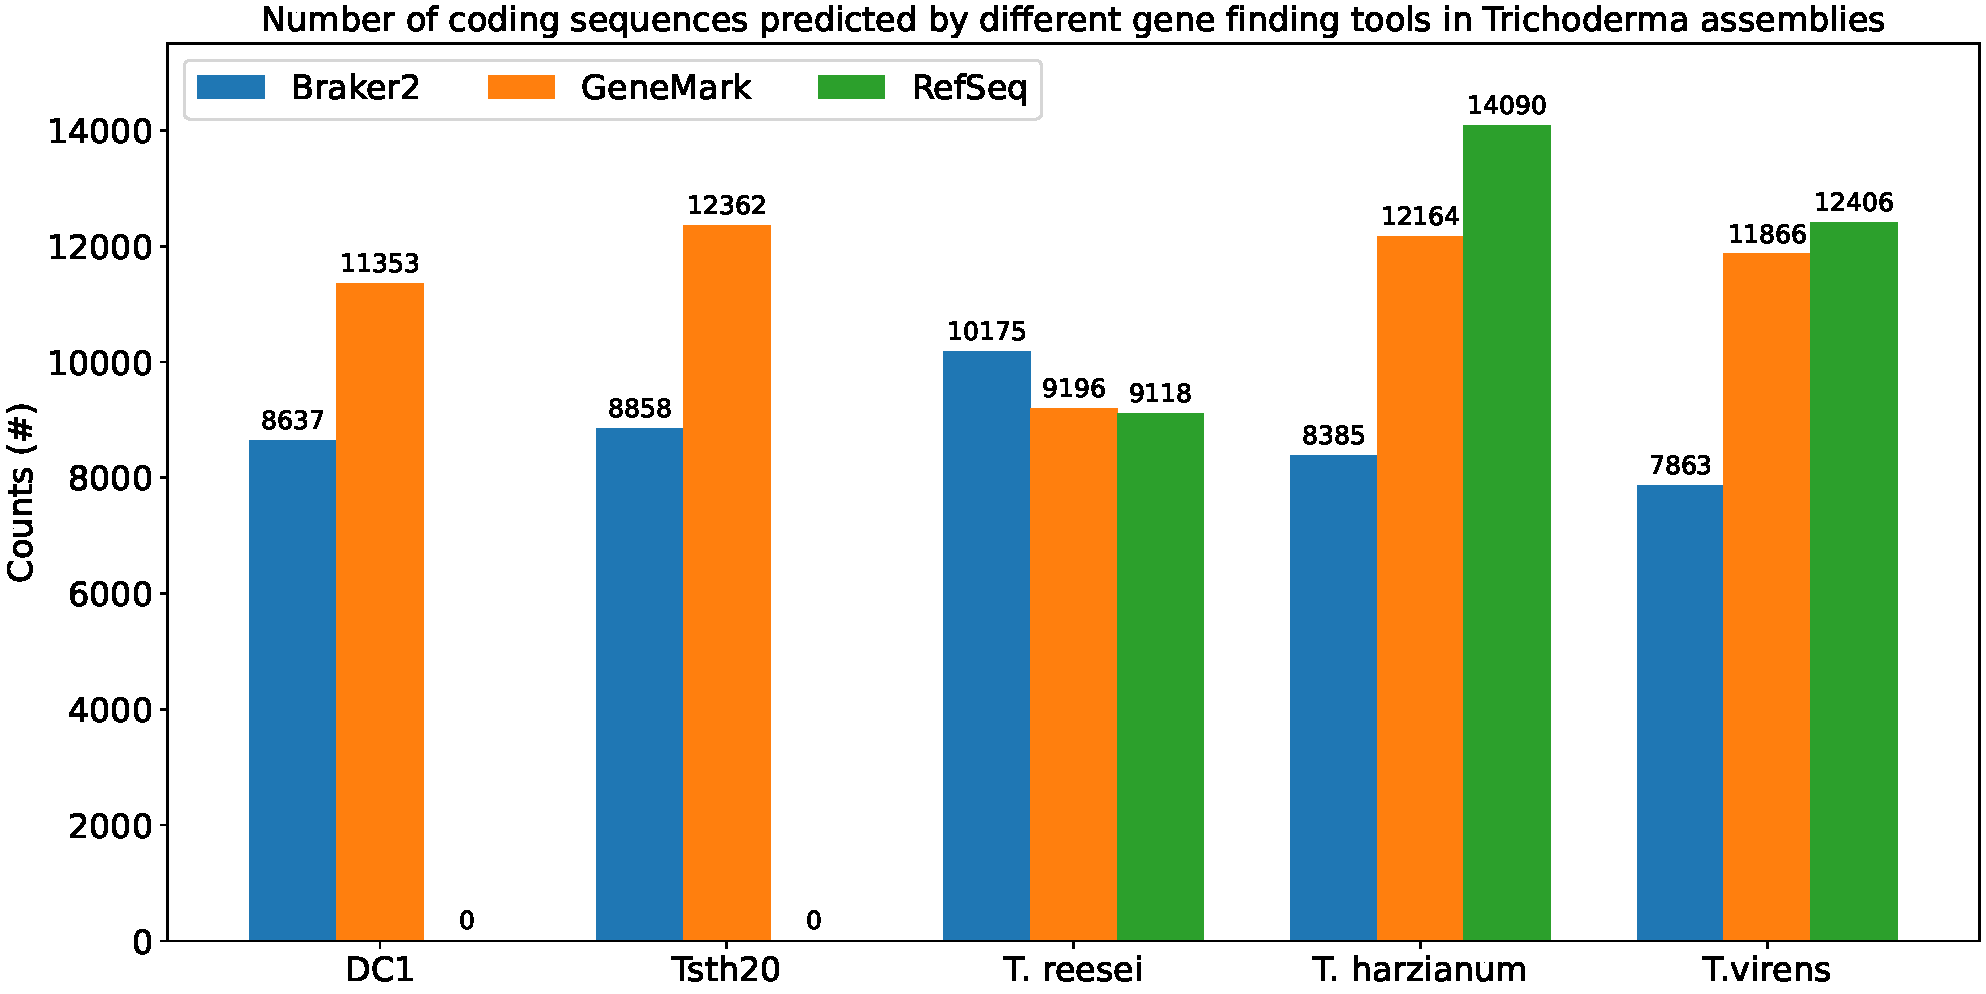
\includegraphics[width=0.9\textwidth]{figures/cds-counts-barplot.pdf}
  \caption[Number of coding sequences predicted]{Number of coding sequences predicted by each gene finder for each \textit{Trichoderma} genome assembly.}\label{fig:cds-counts}
\end{figure}

\begin{table}
  \centering
  \begin{tabular}{|c|c|c|c|c|c|c|}
    \hline
    Assembly & Braker2 & & GeneMark & & RefSeq & \\ \hline
     & Genes & CDS & Genes & CDS & Genes & CDS \\ \hline
    DC1 & 8546 & 8637 & 11353 & 11353 & N/A & N/A \\ \hline
    Tsth20 & 8784 & 8858 & 12362 & 12362 & N/A & N/A \\ \hline
    \textit{T. reesei} & 9659 & 10175 & 9196 & 9196 & 9109 & 9118 \\ \hline
    \textit{T. harzianum} & 8314 & 8385 & 12164 & 12164 & 14269 & 14090 \\ \hline
    \textit{T. virens} & 7801 & 7863 & 11866 & 11866 & 12405 & 12406 \\ \hline
  \end{tabular}
  \caption[Number of genes and coding sequences predicted]{Number of genes and coding sequences
    (isoforms) predicted by each gene finder for each
    \textit{Trichoderma} genome.}\label{table:gene-counts}
\end{table}


